\documentclass[10pt, a4paper]{article}

\usepackage{geometry}
\usepackage{amsmath}
\usepackage{graphicx}
\usepackage{booktabs}

\title{\textbf{HW3 - Generalized Linear Models}}
\author{Vanja Stojanovi\'c}
\date{April 2026}

\begin{document}
\maketitle

\section{Model Implementation}

We implement multinomial and ordinal logistic regression in two ways and compare them.

\subsection{Autograd + gradient descent}

We built a scalar autograd engine (the \texttt{Value} class) supporting addition, multiplication, power, exp, and log, each with a \texttt{\_backward} closure that implements the chain rule. Backpropagation walks a topological sort of the computation graph in reverse. Both models are trained by constructing the negative log-likelihood from \texttt{Value} operations and calling \texttt{backward()} to obtain gradients, then updating parameters with vanilla gradient descent.

\subsection{Optimization library}

We use \texttt{scipy.optimize.fmin\_l\_bfgs\_b} with numerical gradients (\texttt{approx\_grad=True}). The same negative log-likelihood is computed with NumPy arrays. No manual gradient derivation or autograd is needed.

\subsection{Comparison}

\begin{table}[h]
\centering
\begin{tabular}{lcc}
\toprule
 & Autograd + GD & L-BFGS-B (scipy) \\
\midrule
Multinomial fit time & 0.36\,s & 0.003\,s \\
Ordinal fit time     & 0.24\,s & 0.003\,s \\
\bottomrule
\end{tabular}
\end{table}

\textbf{Speed.} L-BFGS-B is roughly 100$\times$ faster. The scalar autograd has Python-level overhead per operation, whereas L-BFGS-B uses vectorized NumPy and a compiled optimizer with second-order curvature information.

\textbf{Convergence.} L-BFGS-B converges more reliably in fewer iterations thanks to approximate Hessian information. The autograd approach requires manual tuning of learning rate and epoch count; too large a step diverges, too small is slow.

\textbf{Numerical stability.} Both require the same softmax/sigmoid stability tricks (subtracting max, clipping probabilities). The autograd version is more fragile for ordinal regression, if thresholds are not initialized with proper spacing, intermediate probabilities become zero and \texttt{log} fails.

\textbf{Prediction similarity.} On the test data, predictions differ by at most 0.003 (multinomial) and 0.016 (ordinal), indicating both converge to similar optima.

\textbf{Implementation difficulty.} The autograd version requires substantially more code (building the \texttt{Value} class, manual training loop). The scipy version is compact, and of course already written for us.

\section{Application}

\subsection{Multinomial Regression on Basketball Shots}

We fit multinomial logistic regression on the basketball dataset (5024 shots, 6 shot types) using one-hot encoded categoricals and standardized continuous features. We estimated coefficient uncertainty via 20 bootstrap resamples; coefficients marked below are those where $|\hat{\beta}| > 2 \cdot \text{SE}$.

\textbf{Key findings:}

\begin{itemize}

\item \textbf{TwoLegged} is the strongest predictor. Two-legged shots strongly favor layups ($+5.7$) and dunks ($+4.1$) over hook shots ($-3.6$) and above-head ($-3.9$). This makes sense biomechanically: layups culminate in a two-footed gather, while hook shots are executed on one foot with a sweeping motion.

\item \textbf{Movement} has large effects. Stationary play (no movement) massively increases hook shots ($+8.7$) and decreases layups ($-10.1$). Driving strongly favors layups ($+3.9$) and reduces above-head shots ($-5.1$). Players who drive to the basket finish close-range with layups; stationary post players use hooks.

\item \textbf{Distance} separates shot types clearly. Farther shots favor above-head ($+4.0$) and other ($+3.8$), while close range favors tip-ins ($-6.1$) and dunks ($-3.1$). This is intuitive: you can only dunk or tip-in right at the rim.

\item \textbf{Competition level}: U14 players almost never dunk ($-5.2$) or tip-in ($-4.8$), younger players lack the height and strength for these shots. They rely more on above-head shots ($+2.6$) and layups ($+2.9$).

\item \textbf{Angle} has a modest effect: higher angles (more lateral) favor layups ($+0.37$) and disfavor tip-ins ($-0.30$). Shots from directly in front are less likely to be layups.

\item \textbf{Transition} increases dunks ($+0.67$) and decreases hook shots ($-0.66$), fast breaks create easy close-range finishes rather than deliberate post moves.

\end{itemize}

Overall, the physical context (distance, stance, movement) dominates shot type selection, while competition level captures physical development differences.

\subsection{Ordinal Regression: When It Outperforms Multinomial}

Ordinal regression outperforms multinomial when the true data-generating process respects the proportional odds assumption: a single latent score shifts probability mass across ordered classes via shared thresholds.

\textbf{Example DGP}: Let $x \sim \mathcal{N}(0, 1)$ and $z = 2x + \varepsilon$ with $\varepsilon \sim \mathcal{N}(0, 0.5)$. Assign classes via thresholds: $y = 0$ if $z < -1$, $y = 1$ if $-1 \le z < 1$, $y = 2$ if $z \ge 1$.

Here the ordinal model matches the DGP exactly (one $\beta$, two thresholds), while multinomial wastes parameters fitting $K$ separate weight vectors. With limited data (small $n$), multinomial overfits while ordinal generalizes better. The advantage grows with more classes $K$, since multinomial needs $O(pK)$ parameters vs.\ ordinal's $O(p + K)$.

The function \texttt{multinomial\_bad\_ordinal\_good} in \texttt{solution1.py} implements this generator.

\section{GLM Diagnostics}

We fit a simple linear regression predicting Distance from Angle and produced three diagnostic plots (Fig.~\ref{fig:diag}). The model is extremely poor ($R^2 = 0.003$), and the diagnostics confirm this.

\begin{figure}[h]
\centering
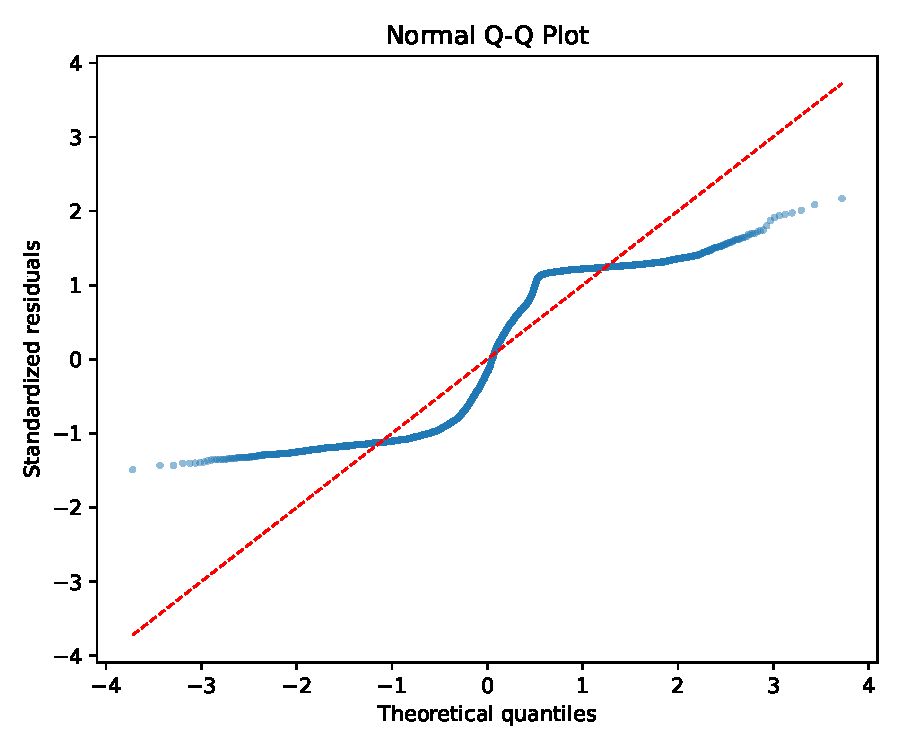
\includegraphics[width=0.48\textwidth]{build/diag_qq.pdf}
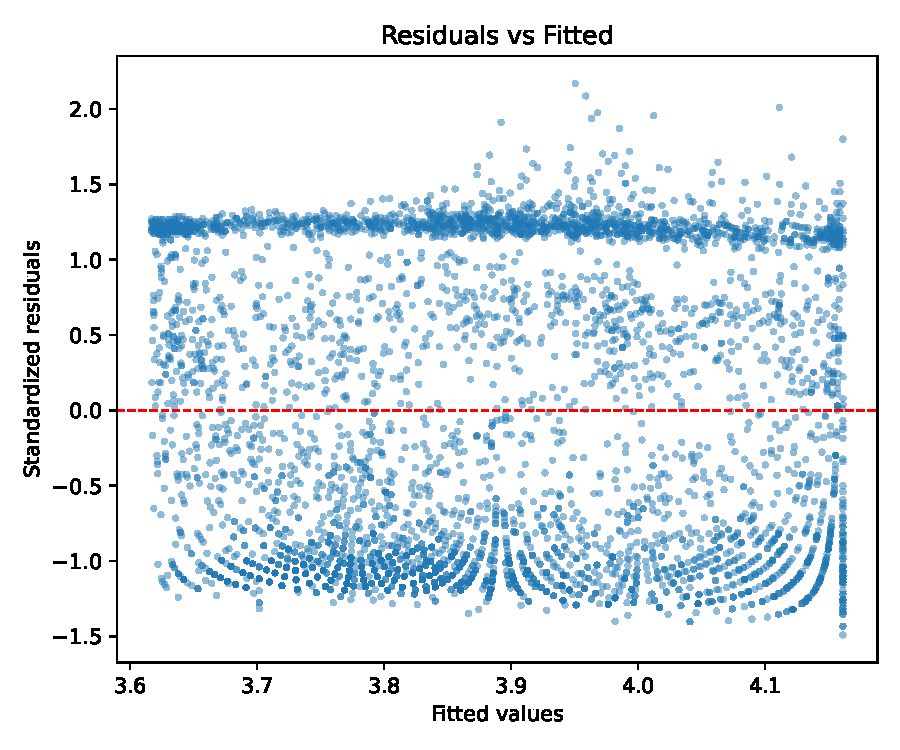
\includegraphics[width=0.48\textwidth]{build/diag_resid_vs_fitted.pdf}
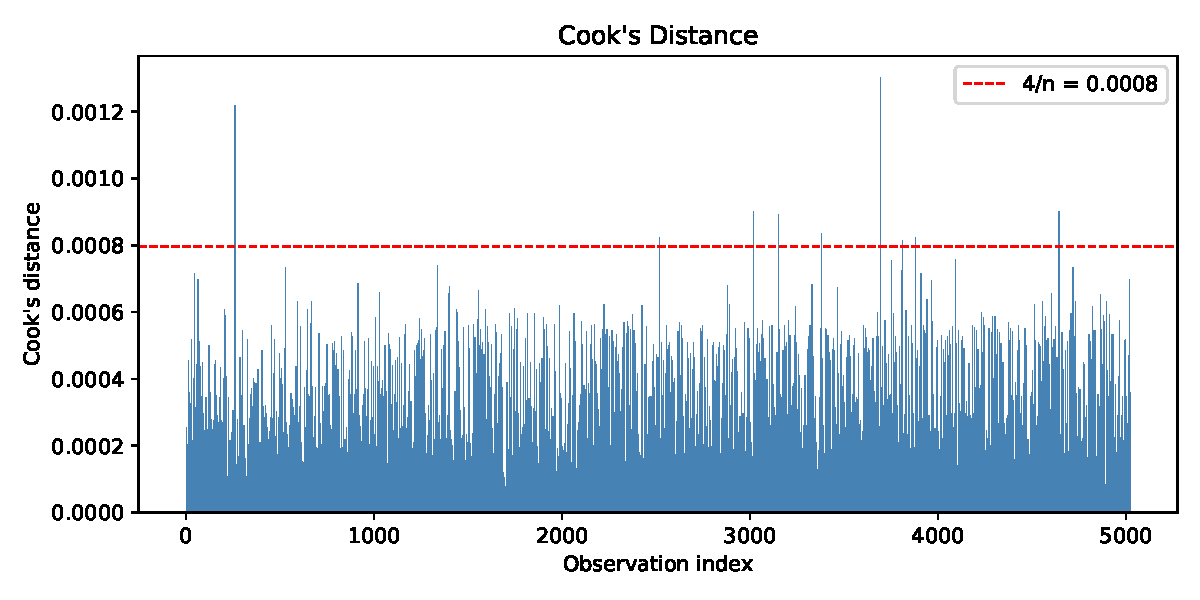
\includegraphics[width=0.6\textwidth]{build/diag_cooks.pdf}
\caption{Diagnostic plots for Distance $\sim$ Angle.}
\label{fig:diag}
\end{figure}

\textbf{Q-Q plot}: Heavy S-shape departure from the diagonal. The left tail flattens (residuals clipped around $-1.2$) and the right tail curves below the line. The residuals are clearly non-normal: the response (distance) is bounded below by 0 and right-skewed, which a normal linear model cannot capture.

\textbf{Residuals vs fitted}: Two distinct horizontal bands are visible rather than random scatter. The upper band near $+1.2$ and the lower spread indicate the response has a multimodal or discrete-like structure (distance values cluster at certain ranges depending on shot type). The banding pattern also shows heteroscedasticity: the spread is not constant across fitted values.

\textbf{Cook's distance}: No single observation dominates the fit; all Cook's distances are below 0.0013, well under the threshold of 1. Nine observations exceed $4/n = 0.0008$, but their influence is negligible. This is expected with $n = 5024$: individual points have little leverage in large samples.

\textbf{Conclusion}: The diagnostics indicate that the linear model is severely misspecified. The near-zero $R^2$, non-normal residuals, and banded residual structure all suggest that the Angle-Distance relationship is not linear, and that Distance's distribution violates the normality assumption of ordinary linear regression.

\end{document}
